\chapter{Softwarová analýza}

Bude zapotřebí hlavní program (nepoptřebujující GUI), který bude zpracovávat data získaná ze senzorů a ty pak kontrolovat, zda jsou spravné. Poté přes konfigurační soubor bude periodicky načítat chtěnou hodnotu, kterou porovná s daty ze senzoru a nastaví je na světlech. Mezitím bude periodicky posílat přes UDP protokol data pro vizualizaci (vlastní komunikační protokol, který bude obsahovat, hodnoty konfiguračního souboru, poslední data ze senzorů, boolean podezření poruchy senzoru a port pro příjem dat k ovládaní přes vizualizaci).

K aplikaci budou mít přístup dva typy lidí -- administrátor a uživatel. Na nejnižší úrovni je uživatel, který může pouze sledovat stavy světel a senzorů. Správce (technik) navíc může vypínat a zapínat celkové osvětlení, upravovat config soubor a manuálně nastavovat intenzitu osvětlení (viz \autoref{Obr-Use_Case_Diagram}). 


Seznam funkcí, které aplikace umí:

\begin{itemize}
    \item sběr procentuálních hodnot osvětlení
    \item sběr viditelnosti ze senzorů
    \item sběr požadovaných procentuálních hodnot skrz vizualizaci
    \item posílaní a následné nastavení chtěné intenzity světla
    \item kontrola senzorů - vždy po sběru dat senzorů
    \item posílaní aktualního stavu vizualizaci
    \item výpočet chtěné intenzity: vezme chtěnou základní hodnotu s configu a upraví ji podle dat získaných senzory 
    \item nastavení config souboru pomocí vizualizace
    \item ukladání dat
    \item kontrola přihlášení od vizualizace.
    \item přepočítaní intenzity (zavolané vizualizací čí změnou config souboru)
\end{itemize}

\section{Komunikace}

V našem projektu jsme se rozhodli využít převážně protokol UDP (User Datagram Protocol), jelikož je jedním z často používaných protokolů v komunikaci a podporuje ho tak námi zvolené prostředí pro vizualizaci i náš hlavní program. Ke zvážení je i možnost využití protokolu TCP (Transmission Control Protocol), který by zaručil spolehlivost doručení dat. Z hlediska rychlosti by nás neomezoval, protože interval mezi posílanými daty není natolik malý, aby došlo k přetížení komunikace. \parencite{TCP_UDP} \parencite{UDP}

\subsection{UDP}

 UDP je základním protokolem modelu TCP/IP. Tento protokol je využíván v případě potřeby rychlé komunikace mezi zařízeními, kde není prioritou doručení veškerých dat. Jeho rychlost spočívá v menší hlavičce paketu, kde oproti protokolu TCP chybí potvrzení o přijetí či možnost obnovení v případě ztráty paketu. Díky tomu hlavička paketu zabírá pouhých 8 B, narozdíl od 20 - 60 B u paketu TCP. UDP navíc funguje jako multicast, což znamená, že může komunikovat s více zařízeními najednou.\parencite{TCP_UDP} \parencite{UDP}

V hlavičce paketu se nachází pouze port odesílajíciho a přijímajícího zařízení, délka paketu a bitový součet (viz \autoref{Obr-UDPPaket}). \parencite{TCP_UDP} \parencite{UDP}

\begin{figure}[H]
    \centering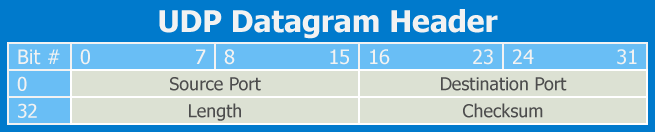
\includegraphics[width=.8\textwidth]{Figures/UDPPaket.png}   
    \caption{Hlavička UDP paketu}
    \label{Obr-UDPPaket}
\end{figure}

\subsection{Způsob komunikace}

\autoref{Obr-Komunikace} nám popisuje komunikaci našeho řešení pro osvětlení parkoviště. Senzory posílají na hlavní PC analogovou proudovou hodnotu. Pomocí drátového UDP protokolu posílají světla aktuální hodnoty na hlavní PC, který zpětně je schopný přes UDP světla ovládat a nastavovat tedy jejich hodnotu svítivosti. Dále je schopen komunikovat s PC uživatele, který má naší aplikaci vytvořenou v prostředí PROMOTIC, případně se servisním PC, a to bezdrátově (wifi). Dále existuje možnost pomocí Node.js komunikace s mobilním telefonem, kterou momentálně nevyužíváme.

\begin{figure}[H]
    \centering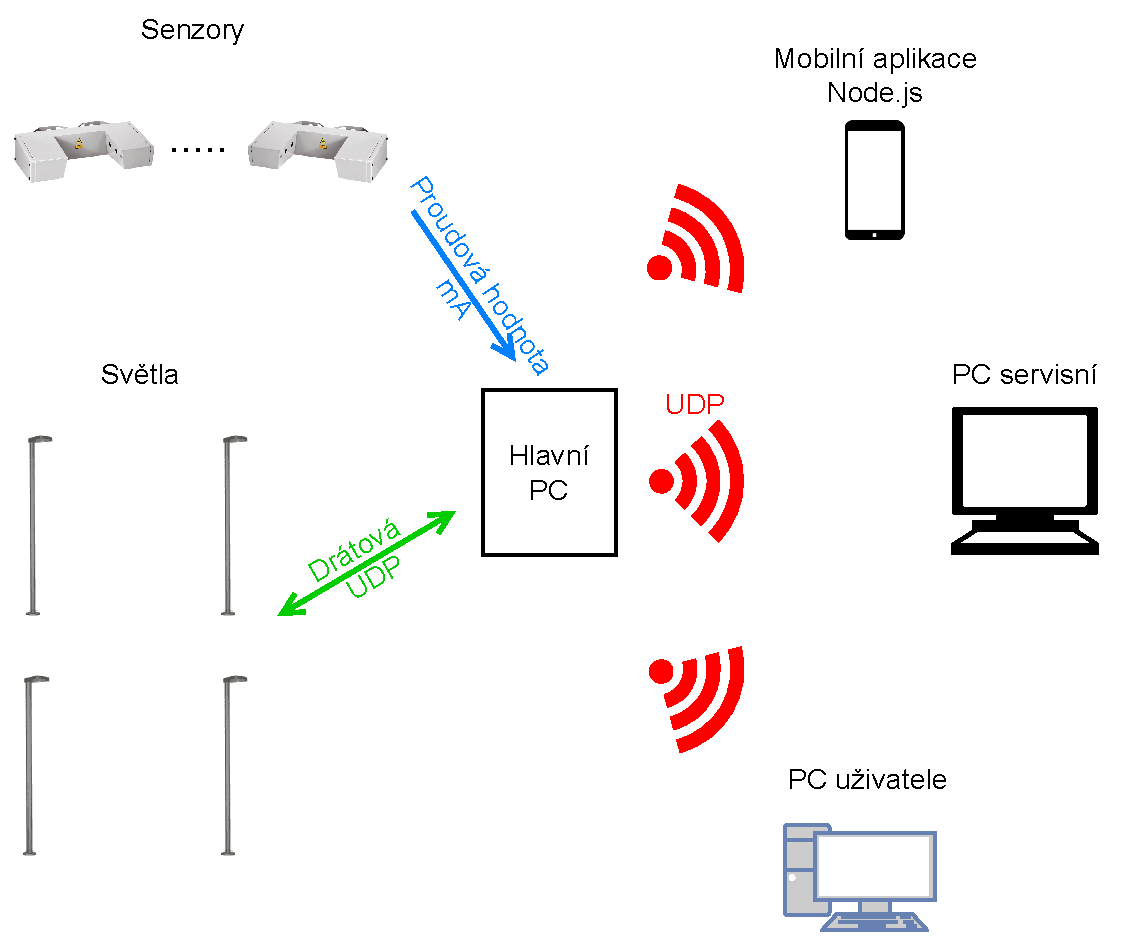
\includegraphics[width=.8\textwidth]{Figures/udp.drawio.pdf}   
    \caption{Komunikace s vizualizací přes UDP}
    \label{Obr-Komunikace}
\end{figure}

\section{Analýza dokumentů}

V naší aplikaci se budou používat tyto soubory:
\begin{itemize}
    \item Config soubor
    \item Usage log
    \item Data log
    \item Error log
\end{itemize}

\textit{Konfigurační soubor} bude posílat každou hodinu hodnoty v procentech, na základě které se stanoví žádaná intenzita. \textit{Usage log} bude zapisovat každé připojení do vizualizace, včetně všech úprav, které se v ní vytvoří. V \textit{Data logu} budou veškerá naměřená data ze senzorů, včetně nastavených procentuálních hodnot svítivosti lamp. Pro zápis chyb vygenerovaných programem budou v souboru \textit{Error log}. Může se jednat třeba o oznámení chybné hodnoty jednoho ze senzorů.

\section{Analýza obsahu a struktury informací}

V hlavním programu budeme využívat dva objekty (třídy), a to pro světla a senzory, přičemž každý z nich bude mít nějaké vlastnosti:

\underline{Objekt světla}
\begin{itemize}
    \item ID světla
    \item intenzita nastavená
    \item stav on/off
\end{itemize}

\underline{Objekt senzoru}
\begin{itemize}
    \item ID senzoru
    \item viditelnost
    \item porucha
\end{itemize}

Viditelnost se porovnává vždycky v určeném časovém úseku (co deset minut) přitom se vyhodnotí případná porucha senzoru. Poté přijde vždy nastavení intenzity, pokud se liší s předchozí hodnotou. Data se budou uchovávat jeden měsíc.

\section{Analýza toku informací}

Tok mezi funkcemi jako takovými moc neřešíme. Pracujeme s globálními hodnotami, uloženými v config souboru. Z hlavního PC vychází již pouze hodnoty, avšak napadnutelné budou přenosy dat mez PC a světly, senzory a vizualizací. Na senzoru snímáme proudový výstup. 

Co se týká ochrany dat přes UDP komunikaci, tak je třeba mít oddělenou síť, protože je relativně snadno přístupná jakýmkoliv zařízením na síti. Data je třeba šifrovat, alespoň posunutím bitů o určitou hodnotu. Dostačující je například kódování spojením hodnot a převrácením bitů, alespoň tedy jako prvotní ochrana.


\section{Analýza slabých míst}

\begin{itemize}
    \item bylo by vhodné zakódování dat, aby nebyly lehce čitelné útoky kdy se sledují pakety na síti
    \item vyhnout se připojení k veřejné síti
    \item nejsme schopni určit správné nastavení hodnot svítivosti světel -- vhodnost zavedení zpětné vazby při jejich nastavování 
    \item nemodulárnost vizualizace
    \item UDP neobsahuje potvrzovací bit -- případně využít protokolu TCP
    \item administrátor zapomene heslo, nemožnost změny hesla
\end{itemize}


\endinput
